\documentclass{article}

\title{AI5006 - Assignment 1}
\author{RVC Sairam - AIRESCH13001 }
\date{September-05-2020}
\usepackage{geometry}
 \geometry{
 a4paper,
 total={170mm,257mm},
 left=20mm,
 top=5mm,
 }
\usepackage{graphicx}
\begin{document}
\maketitle
\section*{Question :}
\large{Find the distance between the two planes
(2 3 4)x = 4 and (4 6 8)x = 12}
\section*{Solution :}
\large{The given two planes are parallel as the perpendicular vectors of the planes (2 3 4) and (4 6 8) are proportional.}\\

\Large{i.e, \( \frac{2}{4} \) = \( \frac{3}{6} \) = \( \frac{4}{8} \)}  \\ \\
\large{Given two parallel planes P1:ax+by+cz+d1=0 and P2:ax+by+cz+d2=0, We can find the distance between these parallel planes using the formula : }\\

\[  \frac{\mid d1 - d2 \mid}{\sqrt{a^2 + b^2 + c^2}}  \] \\

So, the distance between the planes is : \\

\(  \frac{\mid 8 - 12 \mid}{\sqrt{16+36+64}}   = \frac{2}{\sqrt{29}}\)}\\ \\

\begin{center}
    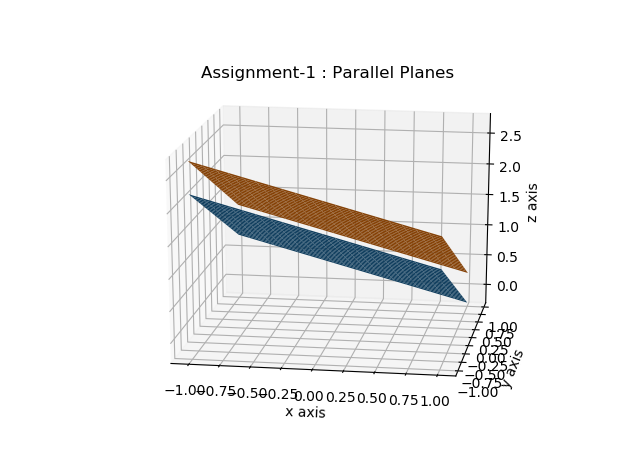
\includegraphics[width = .6\textwidth]{parallel planes.png}
\end{center}

   
\end{document}
